% Based on bare_jrnl_new_sample4.tex from the supplied IEEE template archive.
% Compile with XeLaTeX from this directory.
\documentclass[letterpaper,journal]{IEEEtran}
\usepackage{fontspec}
\usepackage{polyglossia}
\setdefaultlanguage{greek}
\setotherlanguage{english}
\setmainfont{FreeSerif}
\setsansfont{FreeSans}
\setmonofont[Scale=0.80]{DejaVu Sans Mono}
\newfontfamily\greekfont{FreeSerif}
\newfontfamily\greekfontsf{FreeSans}
\newfontfamily\greekfonttt[Scale=0.80]{DejaVu Sans Mono}
\usepackage{amsmath,amssymb}
\usepackage{graphicx,booktabs,array}
\usepackage{xcolor}
\usepackage{tikz}
\usetikzlibrary{arrows.meta,positioning,calc,fit,backgrounds}
\usepackage{listings}
\usepackage{url}
\usepackage[hidelinks,unicode]{hyperref}
\definecolor{navy}{HTML}{17395C}
\definecolor{teal}{HTML}{147D83}
\definecolor{amber}{HTML}{B16C13}
\definecolor{softblue}{HTML}{EDF4FA}
\definecolor{softteal}{HTML}{E9F5F3}
\definecolor{softgray}{HTML}{F5F6F7}
\lstset{language=Python,basicstyle=\ttfamily\scriptsize,
  keywordstyle=\color{navy}\bfseries,commentstyle=\color{teal},
  stringstyle=\color{amber},showstringspaces=false,breaklines=true,
  columns=fullflexible,keepspaces=true,frame=single,rulecolor=\color{black!20},
  backgroundcolor=\color{softgray},numbers=left,numberstyle=\tiny\color{black!50},
  numbersep=5pt,xleftmargin=1.2em,framexleftmargin=0.4em,
  aboveskip=8pt,belowskip=8pt}
\renewcommand{\abstractname}{Περίληψη}
\renewcommand{\IEEEkeywordsname}{Λέξεις κλειδιά}
\renewcommand{\figurename}{Σχήμα}
\renewcommand{\tablename}{Πίνακας}
\renewcommand{\refname}{Βιβλιογραφία}
\newcommand{\code}[1]{\texttt{#1}}
\newcommand{\R}{\mathbb{R}}
\newcommand{\train}{\mathrm{train}}
\newcommand{\test}{\mathrm{test}}
% Populated only from measured benchmark artifacts.


\begin{document}
\title{Σύγκριση ταξινομητών 1-NN, 3-NN και NCC\\στο σύνολο εικόνων CIFAR-100}
\author{Ενδιάμεση εργασία\;—\;Νευρωνικά Δίκτυα και Βαθιά Μάθηση}
\markboth{Νευρωνικά Δίκτυα και Βαθιά Μάθηση — Ενδιάμεση Εργασία}%
{Σύγκριση ταξινομητών στο CIFAR-100}
\maketitle

\begin{abstract}
Η εργασία συγκρίνει τους ταξινομητές πλησιέστερου γείτονα με έναν και τρεις
γείτονες (1-NN και 3-NN) με τον ταξινομητή πλησιέστερου κέντρου κλάσης (NCC).
Χρησιμοποιείται το CIFAR-100, με 50\,000 εικόνες εκπαίδευσης και 10\,000 εικόνες
ελέγχου, και ως χαρακτηριστικά διατηρούνται οι 3\,072 τιμές RGB κάθε εικόνας.
Παρουσιάζονται η οργάνωση των δεδομένων, η μετατροπή σε αριθμούς κινητής
υποδιαστολής, η κλιμάκωση στο $[0,1]$, οι κανόνες ταξινόμησης και η μέτρηση
της ορθότητας. Η αρχική, απλή υλοποίηση διατηρείται ως αναφορά και συγκρίνεται
με ξεχωριστή βελτιστοποιημένη υλοποίηση CPU. Η βελτιστοποίηση αφορά τον τρόπο
εκτέλεσης των υπολογισμών και όχι την εισαγωγή νέων χαρακτηριστικών ή τη μείωση
του συνόλου εκπαίδευσης. Στο πλήρες σύνολο ελέγχου οι ορθότητες είναι
17,55\%, 17,48\% και 10,04\% αντίστοιχα. Η κοινή αναζήτηση γειτόνων
για τα δύο k-NN ολοκληρώνεται σε 10,32 s στη μετρημένη εκτέλεση CPU.
\end{abstract}

\begin{IEEEkeywords}
CIFAR-100, ταξινόμηση εικόνων, k-NN, πλησιέστερο κέντρο κλάσης,
ευκλείδεια απόσταση, ορθότητα, υπολογιστικό κόστος.
\end{IEEEkeywords}

\section{Στόχος και πειραματική προσέγγιση}
Στόχος είναι η σύγκριση τριών απλών κανόνων ταξινόμησης πάνω στα ίδια δεδομένα.
Το ερώτημα είναι ποιο ποσοστό των εικόνων ελέγχου ταξινομεί σωστά κάθε κανόνας
όταν χρησιμοποιούνται απευθείας οι τιμές των εικονοστοιχείων. Δεύτερο ερώτημα
είναι πώς διαφέρει το υπολογιστικό κόστος ανάμεσα στην αποθήκευση όλων των
παραδειγμάτων, όπως στο k-NN, και στη σύνοψή τους με ένα κέντρο ανά κλάση,
όπως στο NCC.

Δεν εκπαιδεύεται νευρωνικό δίκτυο σε αυτό το παραδοτέο. Επίσης δεν εφαρμόζονται
PCA, αύξηση δεδομένων ή εξαγωγή χαρακτηριστικών από προεκπαιδευμένο μοντέλο.
Έτσι η σύγκριση αφορά συγκεκριμένα τους τρεις ταξινομητές στον ίδιο χώρο RGB.
Οι τιμές $k=1$ και $k=3$ προκύπτουν από την εκφώνηση και δεν επιλέγονται
ύστερα από δοκιμές στο σύνολο ελέγχου.

\section{Το σύνολο δεδομένων και η αναπαράστασή του}
Το CIFAR-100 περιλαμβάνει έγχρωμες εικόνες $32\times32$ εικονοστοιχείων,
κατανεμημένες σε 100 κλάσεις. Σε κάθε κλάση αντιστοιχούν 500 εικόνες
εκπαίδευσης και 100 εικόνες ελέγχου. Οι κλάσεις περιλαμβάνουν ζώα, φυτά,
αντικείμενα, οχήματα και σκηνές. Χρησιμοποιούνται οι λεπτομερείς ετικέτες
\code{fine\_labels}, όχι οι 20 υπερκλάσεις \cite{cifar,krizhevsky}.

Η έκδοση Python διαθέτει αρχεία \code{train}, \code{test} και \code{meta}.
Τα δύο πρώτα περιέχουν εικόνες και ετικέτες, ενώ το τρίτο αντιστοιχίζει τους
αριθμητικούς κωδικούς στα ονόματα κλάσεων. Διατηρείται ο επίσημος διαχωρισμός:
οι εικόνες ελέγχου δεν χρησιμοποιούνται ούτε για τον σχηματισμό των κέντρων
ούτε ως υποψήφιοι γείτονες.

\begin{table}[t]
\caption{Πίνακες εισόδου και ετικετών}
\label{tab:shapes}
\centering\small
\begin{tabular}{@{}lll@{}}
\toprule
Μεταβλητή & Σχήμα NumPy & Περιεχόμενο\\
\midrule
$X_{\train}$ & $(50\,000,3\,072)$ & Εικόνες εκπαίδευσης\\
$y_{\train}$ & $(50\,000,)$ & Κλάση κάθε εικόνας\\
$X_{\test}$ & $(10\,000,3\,072)$ & Εικόνες ελέγχου\\
$y_{\test}$ & $(10\,000,)$ & Πραγματικές κλάσεις\\
\bottomrule
\end{tabular}
\end{table}

\subsection{Από την εικόνα στη γραμμή του πίνακα}
Κάθε εικόνα έχει τρία κανάλια χρώματος, άρα
\begin{equation}
D=32\cdot32\cdot3=3\,072.
\end{equation}
Στο αρχείο δεδομένων οι τιμές έχουν ήδη μετατραπεί σε διάνυσμα: προηγούνται
οι 1\,024 τιμές του κόκκινου καναλιού, ακολουθούν οι 1\,024 του πράσινου και
έπειτα οι 1\,024 του μπλε. Μία γραμμή του $X$ επομένως είναι μία ολόκληρη
εικόνα, ενώ μία στήλη αντιστοιχεί σε συγκεκριμένη θέση και κανάλι. Η τιμή
$y_i$ είναι η κλάση της ίδιας εικόνας στη γραμμή $i$. Το $y$ είναι μονοδιάστατος
πίνακας NumPy, όχι πίνακας με 100 στήλες ούτε κωδικοποίηση one-hot.

\begin{figure*}[t]
\centering
\begin{tikzpicture}[font=\small,>=Latex]
\node[draw=navy,fill=softblue,rounded corners,minimum width=2.8cm,minimum height=2cm,align=center] (im) at (0,0)
{Μία εικόνα RGB\\[3pt]$32\times32\times3$\\[3pt]3\,072 τιμές};
\node[align=center,text=navy] at (6,1.8) {$X_{\train}\in\R^{50\,000\times3\,072}$};
\draw[fill=red!12,draw=black!35] (3,0.55) rectangle (5,1.15);
\draw[fill=green!12,draw=black!35] (5,0.55) rectangle (7,1.15);
\draw[fill=blue!12,draw=black!35] (7,0.55) rectangle (9,1.15);
\node at (4,0.85) {$R_0,\ldots,R_{1023}$};
\node at (6,0.85) {$G_0,\ldots,G_{1023}$};
\node at (8,0.85) {$B_0,\ldots,B_{1023}$};
\draw[fill=softblue,draw=black!35] (3,-0.05) rectangle (9,0.55);
\node at (6,0.25) {δεύτερη εικόνα: ακόμη 3\,072 χαρακτηριστικά};
\draw[draw=black!35] (3,-0.65) rectangle (9,-0.05);
\node at (6,-0.35) {$\vdots$};
\draw[fill=softblue,draw=black!35] (3,-1.25) rectangle (9,-0.65);
\node at (6,-0.95) {εικόνα με δείκτη $49\,999$};
\draw[->,thick,navy] (im.east) -- (2.4,0) -- (2.4,0.85) -- (3,0.85);
\node[align=center,text=teal] at (11.5,1.8) {$y_{\train}$\\σχήμα $(50\,000,)$};
\foreach \a/\b/\c in {0.55/1.15/0,-0.05/0.55/1,-1.25/-0.65/49999}{
\draw[fill=softteal,draw=black!35] (10.2,\a) rectangle (12.8,\b);
}
\node at (11.5,0.85) {$y_0\in\{0,\ldots,99\}$};
\node at (11.5,0.25) {$y_1$};
\node at (11.5,-0.35) {$\vdots$};
\node at (11.5,-0.95) {$y_{49\,999}$};
\draw[->,teal,thick] (9,0.85) -- (10.2,0.85);
\node[align=center,font=\footnotesize,text width=5.8cm] at (6,-1.85)
{Γραμμή $i$: μία εικόνα\\Στήλη $j$: ένα χαρακτηριστικό};
\node[align=center,font=\footnotesize,text width=3.2cm] at (11.5,-1.85)
{Ίδιος δείκτης $i$\\στην εικόνα και στην ετικέτα};
\end{tikzpicture}
\caption{Η σύνδεση εικόνων και ετικετών. Η επιπέδωση αλλάζει την αναπαράσταση,
όχι τις τιμές των εικονοστοιχείων. Για το σύνολο ελέγχου ισχύει η ίδια δομή
με 10\,000 γραμμές.}
\label{fig:matrix}
\end{figure*}

Για την προβολή αντιστρέφεται μόνο η διάταξη: η γραμμή μετασχηματίζεται
αρχικά σε $(3,32,32)$ και στη συνέχεια σε $(32,32,3)$, όπως αναμένει η
\code{imshow}. Η μετατροπή αυτή δεν συμμετέχει στην ταξινόμηση.

\subsection{Προεπεξεργασία}
Οι αρχικές τιμές αποθηκεύονται ως \code{uint8} στο διάστημα $[0,255]$.
Πριν από τις αριθμητικές πράξεις μετατρέπονται σε \code{float32} και
διαιρούνται με 255:
\begin{equation}
\widetilde{x}_{ij}=\frac{\operatorname{float32}(x_{ij})}{255}.
\label{eq:scaling}
\end{equation}
Οι ετικέτες παραμένουν ακέραιοι αριθμοί. Η μετατροπή τύπου αποτρέπει την
αναδίπλωση της μη προσημασμένης αριθμητικής κατά την αφαίρεση και επιτρέπει
την αναπαράσταση κλασματικών τιμών. Η διαίρεση αλλάζει την κλίμακα, π.χ.
$0\mapsto0$, $51\mapsto0{,}2$ και $255\mapsto1$.

Η ίδια συνάρτηση εφαρμόζεται στα δύο σύνολα. Δεν υπολογίζονται παράμετροι
κλιμάκωσης από το test set: το 255 είναι το γνωστό μέγιστο της αρχικής
αναπαράστασης. Σε ακριβή αριθμητική η κοινή αυτή κλιμάκωση διατηρεί τη σειρά
των ευκλείδειων αποστάσεων, επειδή
\begin{equation}
d(\mathbf{x}/255,\mathbf{z}/255)=d(\mathbf{x},\mathbf{z})/255.
\end{equation}
Άρα δεν αναμένεται από μόνη της βελτίωση της ορθότητας του k-NN ή του NCC.

\subsection{Ομαδοποίηση κατά κλάση}
Η αρχική υλοποίηση σχηματίζει το λεξικό \code{points}. Το κλειδί είναι ο
αριθμός κλάσης και η τιμή ένας πίνακας με τις εικόνες της:
\begin{equation}
\code{points}[c]=X_{\train}[y_{\train}=c]
\quad\text{με σχήμα }(500,3\,072).
\end{equation}
Η έκφραση $y=c$ δημιουργεί μία λογική μάσκα: επιλέγονται ακριβώς οι γραμμές
που έχουν την αντίστοιχη ετικέτα. Η ομαδοποίηση χρησιμοποιεί μόνο το σύνολο
εκπαίδευσης.

\section{Οι τρεις ταξινομητές}
\subsection{Ευκλείδεια απόσταση}
Κοινό μέτρο ομοιότητας είναι η ευκλείδεια απόσταση δύο διανυσμάτων:
\begin{equation}
d(\mathbf{x},\mathbf{z})=
\sqrt{\sum_{j=1}^{D}(x_j-z_j)^2}.
\label{eq:distance}
\end{equation}
Κάθε χαρακτηριστικό έχει το ίδιο βάρος. Δεν υπάρχει ειδική μεταχείριση
γειτονικών εικονοστοιχείων, περιγραμμάτων ή σχημάτων. Δύο εικόνες μπορεί
να θεωρηθούν κοντινές λόγω παρόμοιου φόντου ή χρωματισμού, χωρίς να απεικονίζουν
το ίδιο είδος αντικειμένου.

\subsection{1-NN και 3-NN}
Στο k-NN η κλήση \code{fit()} αποθηκεύει τα παραδείγματα εκπαίδευσης.
Δεν υπολογίζονται βάρη και δεν εκτελείται επαναληπτική ελαχιστοποίηση σφάλματος.
Για μία νέα εικόνα υπολογίζονται οι αποστάσεις από όλες τις εικόνες εκπαίδευσης
και επιλέγεται το σύνολο $\mathcal{N}_k(\mathbf{x})$ των $k$ κοντινότερων.
Η πρόβλεψη είναι
\begin{equation}
\widehat{y}=\arg\max_c\sum_{i\in\mathcal{N}_k(\mathbf{x})}
\mathbf{1}[y_i=c].
\end{equation}
Το 1-NN αντιγράφει την κλάση του κοντινότερου παραδείγματος. Το 3-NN
χρησιμοποιεί την πλειοψηφία των τριών κοντινότερων. Οι ψήφοι δεν σταθμίζονται
με την απόσταση.

Στην αρχική έκδοση οι γείτονες ταξινομούνται πρώτα ως προς την απόσταση και
έπειτα ως προς τον αριθμό κλάσης. Οι πίνακες εικόνων εξαιρούνται από το κλειδί
ταξινόμησης, διότι η σύγκρισή τους σε ισοπαλία δεν δίνει μία απλή λογική τιμή.
Αν στο 3-NN εμφανιστούν τρεις διαφορετικές κλάσεις, το \code{Counter} επιλέγει
την πρώτη κλάση στη σειρά των γειτόνων που έχει το μέγιστο πλήθος ψήφων:
συνήθως αυτή του κοντινότερου γείτονα, με την προηγούμενη σύμβαση στις ακριβείς
ισοπαλίες αποστάσεων.

\subsection{Πλησιέστερο κέντρο κλάσης (NCC)}
Για κάθε κλάση $c$ υπολογίζεται το κέντρο
\begin{equation}
\boldsymbol{\mu}_c=\frac{1}{n_c}\sum_{i:y_i=c}\mathbf{x}_i,
\qquad n_c=500.
\end{equation}
Η πράξη \code{mean(axis=0)} παίρνει τον μέσο όρο κάθε στήλης, δηλαδή κάθε
θέσης και καναλιού, πάνω στις εικόνες της κλάσης. Παράγονται 100 διανύσματα
μήκους 3\,072. Η νέα εικόνα ταξινομείται ως
\begin{equation}
\widehat{y}=\arg\min_{c\in\{0,\ldots,99\}}
d(\mathbf{x},\boldsymbol{\mu}_c).
\end{equation}
Ο NCC συγκρίνει συνεπώς μία εικόνα με 100 κέντρα αντί για 50\,000 παραδείγματα.
Η οικονομία αυτή έχει κόστος αναπαράστασης: διαφορετικές εμφανίσεις της ίδιας
κλάσης συνοψίζονται σε έναν μοναδικό μέσο όρο. Σε ακριβή ισοπαλία επιλέγεται
η πρώτη κλάση με την ελάχιστη απόσταση, με τις κλάσεις σε αύξουσα σειρά.

\begin{figure}[t]
\centering
\begin{tikzpicture}[font=\footnotesize,>=Latex,node distance=6mm,
block/.style={draw=navy,rounded corners,fill=softblue,align=center,minimum height=9mm,text width=6.6cm},
smallblock/.style={draw=teal,rounded corners,fill=softteal,align=center,text width=2.8cm,minimum height=12mm}]
\node[block] (load) at (0,0) {Ανάγνωση CIFAR-100 και κοινή προεπεξεργασία};
\node[smallblock] (train) at (-1.8,-1.2) {50\,000 εικόνες\\εκπαίδευσης};
\node[smallblock] (test) at (1.8,-1.2) {10\,000 εικόνες\\ελέγχου};
\node[smallblock] (fit) at (-1.8,-2.7) {Αποθήκευση γειτόνων\\ή υπολογισμός κέντρων};
\node[smallblock] (predict) at (1.8,-2.7) {Πρόβλεψη κλάσης\\για κάθε εικόνα};
\node[block] (score) at (0,-4.2) {Σύγκριση προβλέψεων με $y_{\test}$\\Ορθότητα και οπτικοποίηση};
\draw[->,navy] (load.south) -- +(0,-0.2) -| (train.north);
\draw[->,navy] (load.south) -- +(0,-0.2) -| (test.north);
\draw[->,navy] (train.south) -- (fit.north);
\draw[->,navy] (test.south) -- (predict.north);
\draw[->,navy] (fit.east) -- (predict.west);
\draw[->,navy] (predict.south) -- +(0,-0.3) -| (score.north);
\end{tikzpicture}
\caption{Διαχωρισμός της εκπαίδευσης από την αξιολόγηση. Οι αληθινές ετικέτες
ελέγχου χρησιμοποιούνται για τη βαθμολόγηση των προβλέψεων.}
\label{fig:pipeline}
\end{figure}

\section{Οργάνωση και βελτιστοποίηση του κώδικα}
\subsection{Αρχική έκδοση}
Το \code{src/main.py} χωρίζεται σε συναρτήσεις με διακριτές ευθύνες:
\begin{itemize}
\item \code{load\_dataset}: ανάγνωση των αρχείων και ονομάτων κλάσεων.
\item \code{preprocess\_data}: μετατροπή τύπου, κλιμάκωση και ετικέτες.
\item \code{group\_by\_class}: ομαδοποίηση μόνο των εικόνων εκπαίδευσης.
\item \code{fit\_classifiers}: δημιουργία και προσαρμογή των τριών μοντέλων.
\item \code{evaluate\_classifier}: προβλέψεις και μέτρηση ορθότητας.
\item \code{plot\_predictions}: εικόνες με πραγματική και προβλεπόμενη κλάση.
\end{itemize}
Η \code{main()} συνδέει τα στάδια. Η αξιολόγηση ολοκληρώνεται πριν ανοίξουν
τα παράθυρα γραφημάτων και οι εικόνες χρησιμοποιούν ήδη αποθηκευμένες
προβλέψεις. Έτσι δεν επαναλαμβάνεται η ταξινόμηση για την οπτικοποίηση.

Η αρχική αναζήτηση k-NN είναι εύκολη στην παρακολούθηση αλλά περιέχει έναν
βρόχο Python για κάθε εικόνα εκπαίδευσης και πλήρη ταξινόμηση των αποστάσεων.
Για ολόκληρο το test set, κάθε ανεξάρτητη εκτέλεση k-NN απαιτεί
\begin{equation}
50\,000\cdot10\,000=500\,000\,000
\end{equation}
συγκρίσεις εικόνων, με 3\,072 χαρακτηριστικά ανά σύγκριση. Η εκτέλεση
ξεχωριστά για $k=1$ και $k=3$ επαναλαμβάνει τον ίδιο υπολογισμό αποστάσεων.
Η έκδοση αυτή είναι λειτουργική, αλλά ο μεγάλος χρόνος αποτέλεσε το κίνητρο
για βελτιστοποίηση, όχι ένδειξη αποτυχίας του αλγορίθμου.

\subsection{Ξεχωριστή βελτιστοποιημένη έκδοση}
The file \code{src/optimized.py} introduces
\code{OptimizedKNearestNeighbors} and
\code{OptimizedNearestClassCentroid}, while retaining the original implementation
separately. All training images remain candidates; the search is exhaustive,
not approximate.

For a batch of $B$ test images, squared Euclidean distances use the identity
\begin{equation}
\|\mathbf{x}-\mathbf{z}\|_2^2=
\|\mathbf{x}\|_2^2+\|\mathbf{z}\|_2^2-2\mathbf{x}^{\mathsf T}\mathbf{z}.
\label{eq:fastdistance}
\end{equation}
This is the vector equivalent of the familiar scalar expansion
$(a-b)^2=a^2+b^2-2ab$. Here, $\|\mathbf{x}\|_2^2$ is the sum of the
squared components of $\mathbf{x}$, and $\mathbf{x}^{\mathsf T}\mathbf{z}$
is the dot product, the sum of products of corresponding components.
The left-hand side is the squared distance, rather than the distance itself.

This form lets us calculate distances for a whole batch using efficient
BLAS matrix multiplication to compute the dot products. Squared training
norms are calculated once during \code{fit()} and reused for every batch.
We can also omit the square root because squared distances give the same
nearest-neighbor ordering: taking a square root preserves the order of
nonnegative values.

With batches of $B=128$, the distance matrix has shape
$128\times50\,000$ and occupies about 51.2 MB in \code{float64}.
The code does not construct a three-dimensional difference array of shape
$B\times50\,000\times3\,072$, or retain distances for all 10,000 test images
at once. Batching controls memory; array operations and less work inside
Python loops provide the speed improvement.

Instead of sorting all 50,000 values, \code{partition} finds the distance
of the $k$th nearest example. Only candidates at or below that threshold
are sorted, including all ties at the boundary. Their final order uses
distance, class ID and training-example order. The nearest three neighbors
are sufficient to produce both 1-NN and 3-NN predictions from one search.

The optimized NCC retains the original class-mean calculation and uses the
same distance identity against the 100 centroids. Its class order on exact
distance ties is unchanged.

Inputs are normalized \code{float32} values, while optimized distance
arithmetic uses \code{float64} to reduce cancellation error in
\eqref{eq:fastdistance}. Tiny negative computed squared distances are clipped
to zero. The mathematical distance is unchanged, but bitwise equivalence
with the original arithmetic is not guaranteed; nearly tied distances
require care. Predictions are therefore explicitly compared against the
original implementation.


\section{Αξιολόγηση και αποτελέσματα}
\subsection{Πρωτόκολλο και μετρική}
Όλοι οι ταξινομητές χρησιμοποιούν την ίδια αναπαράσταση και τις ίδιες ετικέτες.
Η ορθότητα (accuracy) είναι
\begin{equation}
A=\frac{1}{N_{\test}}\sum_{i=1}^{N_{\test}}
\mathbf{1}[\widehat{y}_i=y_i].
\end{equation}
Η μετρική αυτή απαντά ποιο ποσοστό των εικόνων αναγνωρίστηκε σωστά. Δεν είναι
η ανά κλάση precision. Εδώ το test set είναι ισοκατανεμημένο στις 100 κλάσεις,
οπότε η συνολική ορθότητα αποτελεί άμεση, εύληπτη βάση σύγκρισης. Ένας κανόνας
που προβλέπει πάντα μία σταθερή κλάση πετυχαίνει ακριβώς $1\%$ στο πλήρες
σύνολο ελέγχου.

Οι χρόνοι πρόβλεψης μετρώνται χωριστά από φόρτωση αρχείων και γραφήματα.
Το μικρό αρχικό πείραμα των 20 εικόνων χρησιμοποιήθηκε μόνο για έλεγχο της
λειτουργίας και του κόστους. Δεν χρησιμοποιείται ως υποκατάστατο της τελικής
σύγκρισης. Η σύγκριση ταχύτητας μεταξύ εκδόσεων απαιτεί ίδιο πλήθος εικόνων
και ίδιο σύνολο εκπαίδευσης. Οι προεκτάσεις χρόνου σημειώνονται ως εκτιμήσεις,
όχι ως πραγματικές πλήρεις εκτελέσεις.

\subsection{Μετρήσεις}
Measurements used an AMD Ryzen 9 7950X CPU, eight OpenBLAS threads,
Python 3.10.12, NumPy 1.24.3 and OpenBLAS 0.3.21. Batch size was 128.
No GPU was used. Each reported prediction time is one wall-clock
measurement after a short warm-up, not an average of repeated runs.
Timings depend on the machine and its concurrent workload.

The common comparison sample contained one test image per class, selected
with \code{default\_rng} and seed 2026: 100 images in total. Every classifier
used all 50,000 training examples. Each optimized model agreed with its
original on \textbf{all 100 predictions}. This validates the sample, not
every possible numerical tie. The original NCC was also run on the entire
test set, yielding agreement on all 10,000 predictions.

\begin{table}[t]
\caption{Full evaluation on 10,000 test images}
\label{tab:accuracy}
\centering\small
\begin{tabular}{@{}lrr@{}}
\toprule
Classifier & Correct predictions & Accuracy\\
\midrule
1-NN & 1\,755 & 17.55\%\\
3-NN & 1\,748 & 17.48\%\\
NCC & 1\,004 & 10.04\%\\
\bottomrule
\end{tabular}
\end{table}

\begin{figure}[t]
\centering
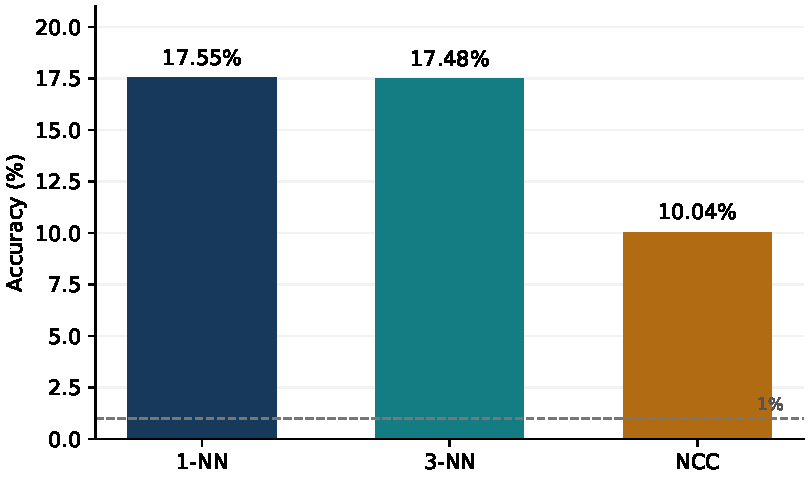
\includegraphics[width=\columnwidth]{figures/accuracy.pdf}
\caption{Measured accuracy of the optimized implementations on the full
test set. The dashed line marks the 1\% achieved by a constant class
prediction on this balanced dataset.}
\label{fig:accuracy}
\end{figure}

\begin{table}[t]
\caption{Prediction time on the same 100-image sample}
\label{tab:timing}
\centering\small
\begin{tabular}{@{}lrrr@{}}
\toprule
Model & Original (s) & Optimized (s) & Speedup\\
\midrule
1-NN & 24.173 & 0.0916 & $263.8\times$\\
3-NN & 24.031 & 0.1095 & $219.5\times$\\
NCC & 0.0417 & 0.000589 & $70.9\times$\\
\bottomrule
\end{tabular}
\end{table}

Table~\ref{tab:timing} uses separate prediction calls for each classifier.
In the final full run, the shared 1-NN/3-NN search took
\textbf{10.319 s} for all 10,000 images. This is the time for
\emph{both results together}, not an independent runtime for each model.
It includes neighbor selection, voting and progress messages.
Optimized NCC prediction took 0.0567 s; the original NCC took 4.158 s
on the same full set.

The original k-NN \code{fit()} only stores a dictionary reference and
was measured at approximately $1\,\mu$s. Shared optimized k-NN preparation
took 1.523 s because it constructs a contiguous \code{float64} matrix,
labels and squared norms. This preparation is paid once and excludes
loading and grouping. NCC centroid construction took about 0.023 s
in both versions.

The original k-NN implementations were not run on the entire test set.
Extrapolating their sample timings suggests about 40 minutes per original
pass; this is an \emph{estimate}, not a measured full run. The original
implementation is functional. The observed CPU acceleration made GPU
support and PCA unnecessary for this experiment.

The files \code{results/cpu\_benchmark.json} and
\code{results/predictions.npz} retain the settings, measurements and full
predictions in original test-set order. The JSON also records sample
indices and SHA-256 hashes of the measured source files.


\subsection{Παραδείγματα ταξινόμησης}
Το Σχήμα~\ref{fig:examples} δείχνει πραγματικές προβλέψεις από την πλήρη
εκτέλεση. Για κάθε ταξινομητή επιλέγονται, με τη σειρά των δεικτών του test
set, οι πρώτες δύο σωστές και οι πρώτες δύο λανθασμένες προβλέψεις.
Η επιλογή είναι αναπαραγώγιμη και δεν αποτελεί τυχαίο ή αντιπροσωπευτικό
δείγμα της συνολικής απόδοσης. Τα ονόματα παραμένουν στην αγγλική μορφή
του CIFAR-100 για άμεση αντιστοίχιση με τα μεταδεδομένα.

\begin{figure*}[t]
\centering
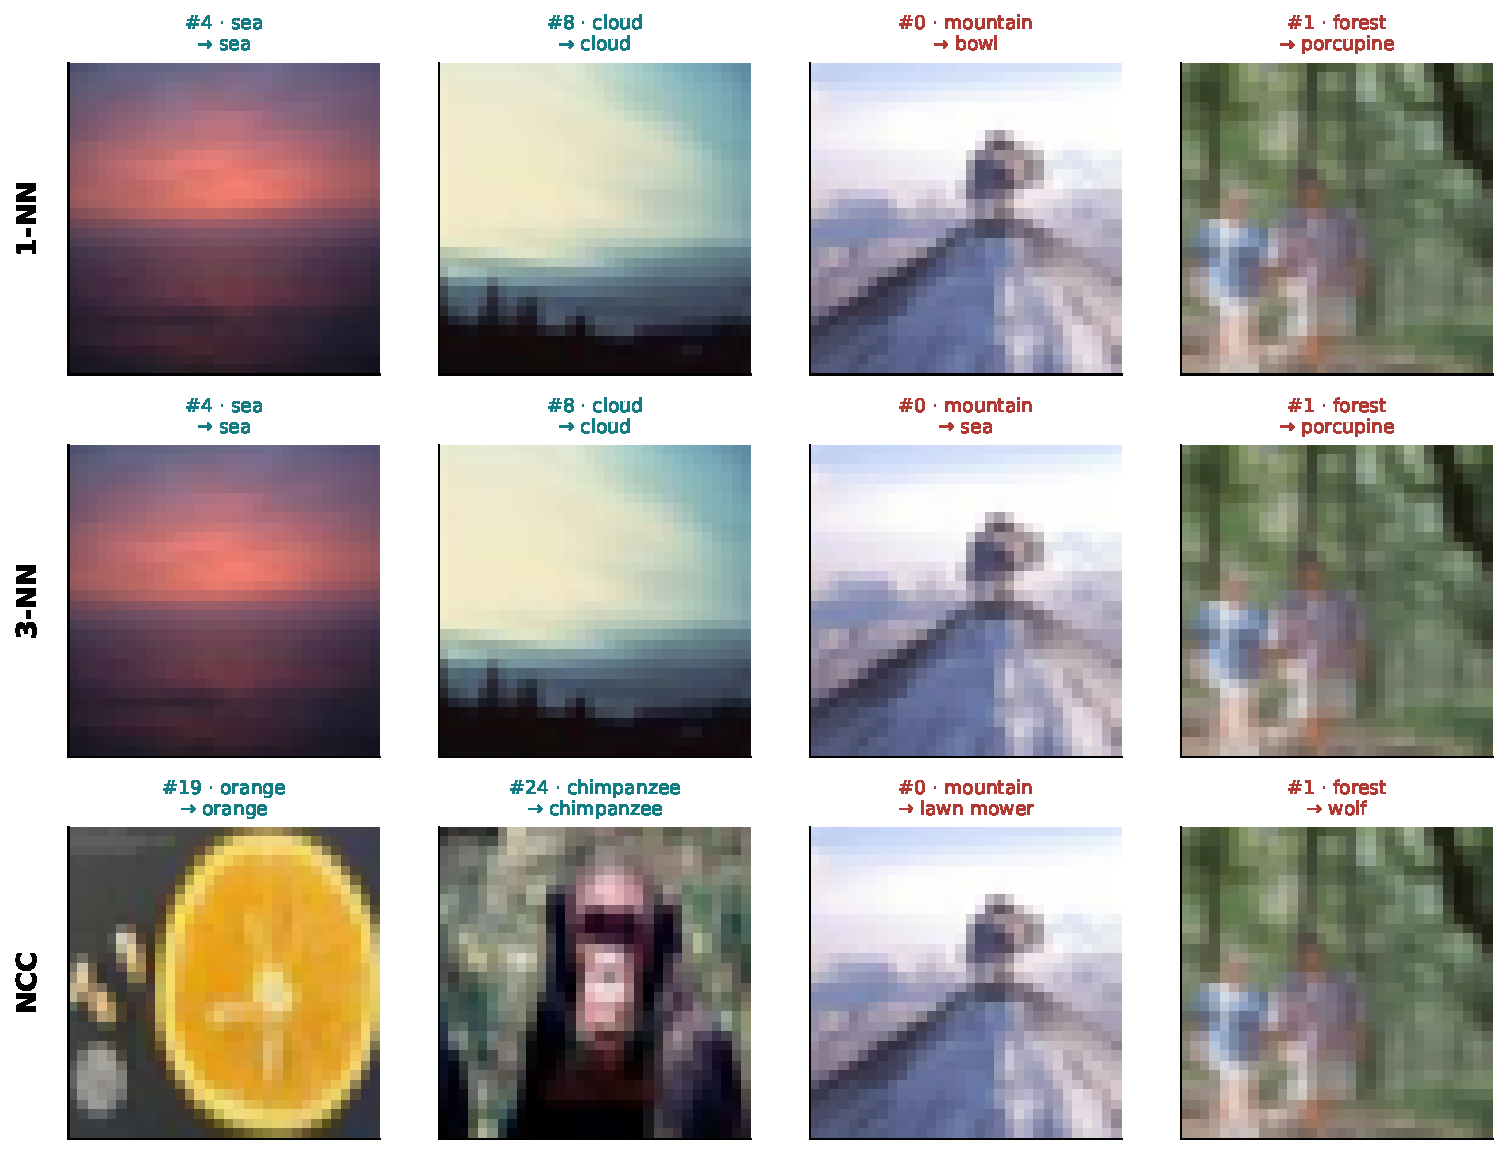
\includegraphics[width=0.95\textwidth]{figures/classification_examples.pdf}
\caption{Μία σειρά ανά ταξινομητή. Οι δύο αριστερές στήλες είναι σωστές
προβλέψεις (πράσινοι τίτλοι), οι δύο δεξιές λανθασμένες (κόκκινοι τίτλοι).
Πάνω από κάθε εικόνα αναγράφονται ο δείκτης στο test set και η πραγματική
κλάση· μετά το βέλος ακολουθεί η πρόβλεψη.}
\label{fig:examples}
\end{figure*}


\section{Συζήτηση και περιορισμοί}
Η ευκλείδεια απόσταση πάνω σε ακατέργαστες τιμές RGB δεν παρέχει αναλλοιωτότητα
ως προς μετατόπιση, προσανατολισμό ή αλλαγές φωτισμού. Η μικρή ανάλυση επίσης
περιορίζει την οπτική πληροφορία. Έτσι, ακόμη και ένα αντικείμενο που είναι
εύκολα αναγνωρίσιμο από άνθρωπο δεν είναι υποχρεωτικά κοντά στα παραδείγματα
της ίδιας κλάσης στον συγκεκριμένο διανυσματικό χώρο.

Το 3-NN μπορεί να περιορίσει την επιρροή ενός μεμονωμένου γείτονα, αλλά δεν
υπάρχει εγγύηση ότι θα ξεπεράσει το 1-NN: οι πρόσθετοι γείτονες μπορεί να
ανήκουν σε άλλη κλάση. Ο NCC μειώνει δραστικά τις συγκρίσεις κατά την πρόβλεψη,
αλλά ένα μόνο κέντρο δεν αποτυπώνει πολλαπλές ομάδες εμφανίσεων της ίδιας
κλάσης. Η μετρημένη σύγκριση αφορά αυτόν τον συνδυασμό δεδομένων,
χαρακτηριστικών και απόστασης και όχι μία γενική κατάταξη των αλγορίθμων.

Τα δεδομένα είναι ένα συγκεκριμένο σύνολο εικόνων αναφοράς και δεν τεκμηριώνουν
απόδοση σε πραγματικές εφαρμογές ή σε εικόνες άλλης προέλευσης. Δεν
πραγματοποιήθηκε ανεξάρτητος έλεγχος κάθε εικόνας για πιθανές ομοιότητες μεταξύ
training και test. Διατηρήθηκε ο επίσημος διαχωρισμός και δεν προστέθηκαν
δεδομένα από προσωπικές συλλογές. Η διάθεση των αρχικών εικόνων διέπεται από
τους όρους της πηγής τους· δεν συνάγεται γενική άδεια επαναχρησιμοποίησης
από τη δυνατότητα λήψης του συνόλου.

\section{Conclusion}
In this experiment, 1-NN achieved 17.55\%, 3-NN 17.48\% and NCC 10.04\%.
The k-NN results are very close: the difference is only seven correct
predictions, or 0.07 percentage points. Without further statistical
analysis, this does not establish general superiority of 1-NN.
Both k-NN models outperformed NCC in this feature space, while NCC had
much lower prediction cost.

The original implementation makes the classification rules and evaluation
pipeline explicit. Full k-NN evaluation posed a practical execution constraint,
so a separate AI-written implementation was used to obtain the reported
accuracies without reducing the training set. Its computational changes are
explained in the appendix, and agreement checks and their limits are stated.
The main result is the accuracy comparison between classifiers, rather than
an implementation speed comparison. The modest accuracy illustrates the
limitations of using raw RGB distances to recognize object classes.


\clearpage
\onecolumn
\lstset{basicstyle=\ttfamily\footnotesize}
\appendices
\section{Αρχική υλοποίηση: κρίσιμα αποσπάσματα}
Τα παρακάτω αποσπάσματα προέρχονται απευθείας από το συνοδευτικό
\code{src/main.py}. Το πλήρες αρχείο περιλαμβάνει επίσης φόρτωση,
προεπεξεργασία, εκτέλεση και γραφήματα.
\begin{minipage}{\linewidth}
\lstinputlisting[firstline=41,lastline=42]{../src/main.py}
\end{minipage}
\begin{minipage}{\linewidth}
\lstinputlisting[firstline=56,lastline=70]{../src/main.py}
\end{minipage}
\begin{minipage}{\linewidth}
\lstinputlisting[firstline=78,lastline=91]{../src/main.py}
\end{minipage}
\begin{minipage}{\linewidth}
\lstinputlisting[firstline=109,lastline=126]{../src/main.py}
\end{minipage}

\clearpage
\section{Βελτιστοποιημένη υλοποίηση: κρίσιμα αποσπάσματα}
These excerpts are taken from the accompanying \code{src/optimized.py}.
The shared distance function is used for both training examples and class
centroids.
\par\noindent\begin{minipage}{\linewidth}
\lstinputlisting[firstline=8,lastline=16]{../src/optimized.py}
\end{minipage}\par
\par\noindent\begin{minipage}{\linewidth}
\lstinputlisting[firstline=59,lastline=70]{../src/optimized.py}
\end{minipage}\par
\par\noindent\begin{minipage}{\linewidth}
\lstinputlisting[firstline=72,lastline=83]{../src/optimized.py}
\end{minipage}\par

Optimized NCC compares each batch against the class centroids using the
same shared distance function:
\par\noindent\begin{minipage}{\linewidth}
\lstinputlisting[firstline=112,lastline=121]{../src/optimized.py}
\end{minipage}\par

The file \code{src/benchmark.py} performs agreement checks, timing and full
evaluation. Complete source files accompany this report.


\begin{thebibliography}{3}
\bibitem{cifar}
A. Krizhevsky, V. Nair και G. Hinton, ``CIFAR-10 and CIFAR-100 datasets.''
\url{https://www.cs.toronto.edu/~kriz/cifar.html}.
\bibitem{krizhevsky}
A. Krizhevsky, \textenglish{\emph{Learning Multiple Layers of Features from
Tiny Images}}, τεχνική αναφορά, University of Toronto, 2009, κεφ.~3.
\url{https://www.cs.toronto.edu/~kriz/learning-features-2009-TR.pdf}.
\bibitem{assignment}
Εκφώνηση πρώτης υποχρεωτικής εργασίας, μάθημα «Νευρωνικά Δίκτυα -- Βαθιά
Μάθηση», ενότητα «Ενδιάμεση Εργασία», 2026.
\end{thebibliography}
\end{document}
